% Binomial tree for three periods. Generated by a short script.
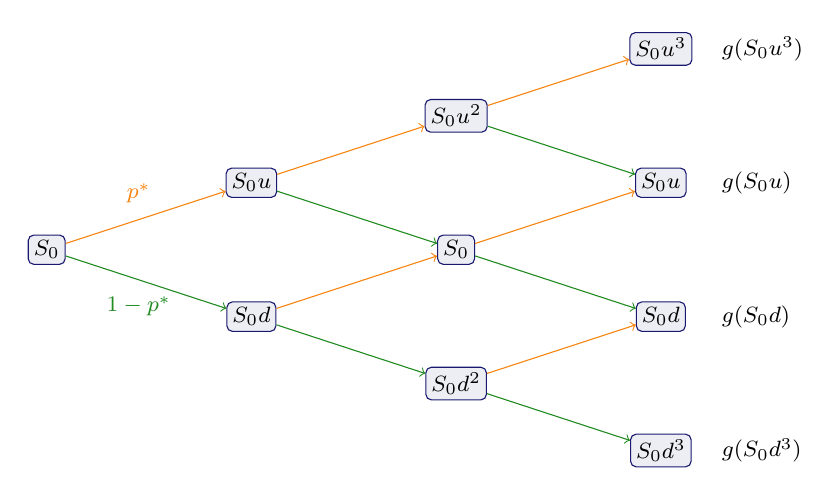
\begin{tikzpicture}[x=2.6cm,y=0.85cm,every node/.style={font=\footnotesize},nd/.style={draw=MidnightBlue,fill=MidnightBlue!8,rounded corners=2pt,inner sep=2pt}]
\node[nd] (n00) at (0,0) {$S_0$};
\node[nd] (n10) at (1,-1) {$S_0d$};
\node[nd] (n11) at (1,1) {$S_0u$};
\node[nd] (n20) at (2,-2) {$S_0d^2$};
\node[nd] (n21) at (2,0) {$S_0$};
\node[nd] (n22) at (2,2) {$S_0u^2$};
\node[nd] (n30) at (3,-3) {$S_0d^3$};
\node[nd] (n31) at (3,-1) {$S_0d$};
\node[nd] (n32) at (3,1) {$S_0u$};
\node[nd] (n33) at (3,3) {$S_0u^3$};
\draw[->,BurntOrange] (n00)--(n11);
\draw[->,ForestGreen] (n00)--(n10);
\draw[->,BurntOrange] (n10)--(n21);
\draw[->,ForestGreen] (n10)--(n20);
\draw[->,BurntOrange] (n11)--(n22);
\draw[->,ForestGreen] (n11)--(n21);
\draw[->,BurntOrange] (n20)--(n31);
\draw[->,ForestGreen] (n20)--(n30);
\draw[->,BurntOrange] (n21)--(n32);
\draw[->,ForestGreen] (n21)--(n31);
\draw[->,BurntOrange] (n22)--(n33);
\draw[->,ForestGreen] (n22)--(n32);
\node[BurntOrange,above] at (0.45,0.55) {$p^*$};
\node[ForestGreen,below] at (0.45,-0.55) {$1-p^*$};
\node[right] at (3.25,-3) {$g(S_0d^3)$};
\node[right] at (3.25,-1) {$g(S_0d)$};
\node[right] at (3.25,1) {$g(S_0u)$};
\node[right] at (3.25,3) {$g(S_0u^3)$};
\end{tikzpicture}
